\documentclass[xcolor=pdftex,dvipsnames]{beamer}

\usepackage{amsmath}
\usepackage{amssymb}
\usepackage{comment}
\usepackage{textcomp}
\usepackage{ulem}
\DeclareRobustCommand{\rsout}[1]{\texorpdfstring{\sout{#1}}}

\title{Microeconomic Theory --- ECON 323 503 \\ Chapter 12: Pricing
\rsout{and Advertising}}
\author{Vikram Manjunath}       %
\institute{Texas A\&M University}
\setbeamertemplate{navigation symbols}{}
\setbeamertemplate{footline}{}
\usefonttheme{serif}
\begin{document}

\maketitle

\begin{frame}
\frametitle{Outline}
\begin{enumerate}[<+->]
\item Price discrimination: A monopoly can increase its profits by
  charging different consumers different prices.
\end{enumerate}
\end{frame}


\begin{frame}
  \frametitle{Price discrimination}
  Previous chapter: monopoly had to set a \emph{uniform} price.\bigskip
  
\uncover<2->{  Often, there are different prices: sales, slightly differentiated
  products, coupons, and so on.\bigskip}

\uncover<3->{    Why do we see these different prices?\bigskip}

\uncover<4->{    More often than not: \emph{price discrimination.}}


\end{frame}

\begin{frame}
  \frametitle{Perfect price discrimination}
  Simplified environment:
  
  \bigskip
\uncover<2->{    Each consumer consumes at most one unit.}

  \bigskip
\uncover<3->{    Monopolist knows exactly what each person's willingness to pay is.}

  \bigskip
\uncover<4->{    Since he can charge each person a different price, selling one
  additional unit doesn't reduce the price of the units he's already
  selling.}
  \bigskip

\uncover<5->{    So  $MR(Q) = p(Q)$!}
  
\end{frame}

\begin{frame}
  \frametitle{Perfect price discrimination}
  \begin{center}
    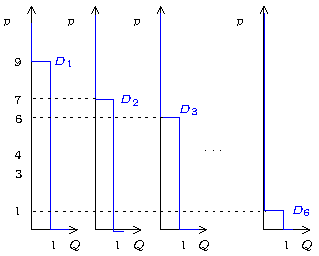
\includegraphics{pics/PriceDiscrimination1}
  \end{center}
Each person's demand curve tells us his willingness to pay for a unit
of the good.
\end{frame}


\begin{frame}
  \frametitle{Perfect price discrimination}
  \begin{center}
    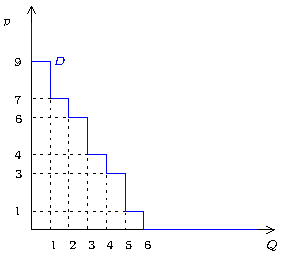
\includegraphics{pics/PriceDiscrimination2}
  \end{center}
Adding them up horizontally gives us the market demand curve.
\end{frame}


\begin{frame}
\frametitle{Perfect price discrimination}
Suppose constant marginal cost of \$4.00
\bigskip

\uncover<2->{  How many units should the monopolist sell? }

\bigskip
\uncover<3->{  How much should he charge each consumer?}

\bigskip
\uncover<4->{  No point selling to anyone who values it less \$4.00: they won't pay
the cost of producing it.}

\bigskip
\uncover<5->{  Sell to anyone who values it at \$4.00 or more and charge them their
willingness to pay.}
\end{frame}

\begin{frame}
\frametitle{Perfect price discrimination}
\begin{center}
  \includegraphics{pics/Pricediscrimination3}
\end{center}
Sell one unit each  to consumers 1, 2,  3, and 4. 
\end{frame}

\begin{frame}
\frametitle{Perfect price discrimination}
\begin{center}
  \includegraphics{pics/Pricediscrimination3}
\end{center}
Charge each their willingness to pay.
\end{frame}

\begin{frame}
\frametitle{Perfect price discrimination}
\begin{center}
  \includegraphics{pics/Pricediscrimination4}
\end{center}
Revenue is the shaded area.
\end{frame}
\begin{frame}
\frametitle{Perfect price discrimination}
\begin{center}
  \includegraphics{pics/Pricediscrimination5}
\end{center}
PS is this shaded area (or profit if no fixed cost)
\end{frame}


\begin{frame}
  \frametitle{Smooth demand curves}

  \begin{center}
    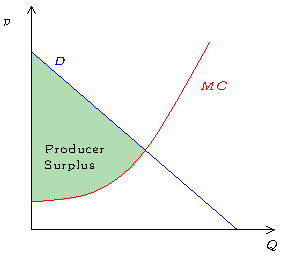
\includegraphics{pics/PriceDiscriminationSmooth}
  \end{center}

The intuition here follows through even for ``smooth''
  demand curves.


\end{frame}


\begin{frame}
  \frametitle{Welfare}
  By discriminating, the monopoly gets \emph{all} of the surplus.

  \bigskip
\uncover<2->{    Social welfare $W=PS+CS$ is what it would be in a competitive
  market: it's efficient.}

  \bigskip
\uncover<3->{    But the consumer is hurt.}

  \bigskip
\uncover<4->{    An example of this: net neutrality prevents internet providers (who are
  typically monopolists) from discriminating.}


\end{frame}





\end{document}








